\section{Results and Discussion}
The following are the precision, recall, F1-score, and support metrics for each classification model, evaluating its performance across six emotion categories: Sadness, Joy, Love, Anger, Fear, and Surprise.

\begin{figure}[h!]
\centering
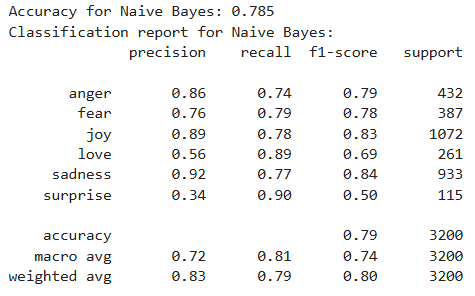
\includegraphics[width=0.8\textwidth]{naive_bayes_result.png}
\caption{Naive Bayes Classification Report}
\label{fig:naive_bayes}
\end{figure}

\begin{figure}[h!]
\centering
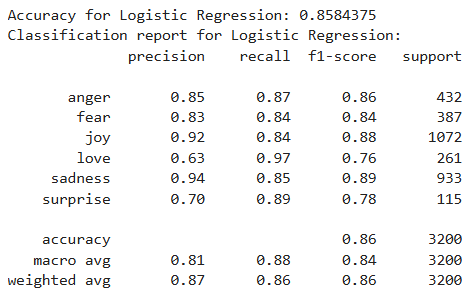
\includegraphics[width=0.8\textwidth]{logistic_regression_result.png}
\caption{Logistic Regression Classification Report}
\label{fig:logistic_regression}
\end{figure}

\begin{figure}[h!]
\centering
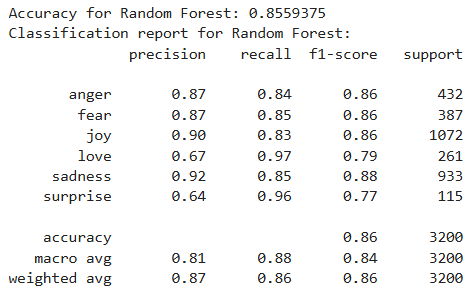
\includegraphics[width=0.8\textwidth]{random_forest_result.png}
\caption{Random Forest Classification Report}
\label{fig:random_forest}
\end{figure}

\begin{figure}[h!]
\centering
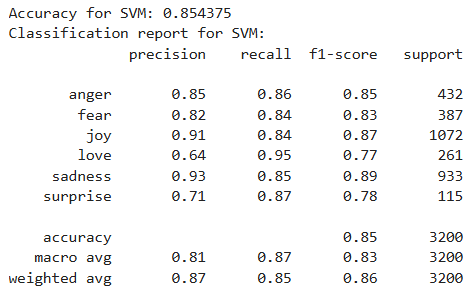
\includegraphics[width=0.8\textwidth]{svm_result.png}
\caption{SVM Classification Report}
\label{fig:svm}
\end{figure}

\begin{figure}[h!]
\centering
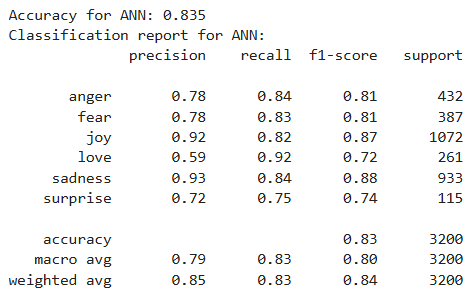
\includegraphics[width=0.8\textwidth]{ann_result.png}
\caption{ANN Classification Report}
\label{fig:ann}
\end{figure}

\begin{figure}[h!]
\centering
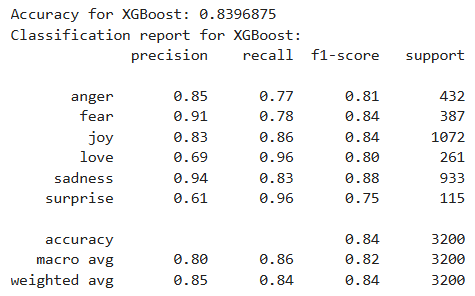
\includegraphics[width=0.8\textwidth]{xgboost_result.png}
\caption{XGBoost Classification Report}
\label{fig:xgboost}
\end{figure}

\clearpage
\subsection{Naive Bayes Result}
The Naive Bayes model achieved an accuracy of \textbf{0.785}. It performed reasonably well across several emotions, with \textbf{Sadness} showing the highest recall (0.77) and \textbf{Surprise} the lowest precision (0.34) as shown in Figure \ref{fig:naive_bayes}. The weighted average F1-score of 0.80 indicates balanced performance across emotions, though some areas like \textbf{Surprise} and \textbf{Love} could be improved. In terms of precision, the model had the best result for \textbf{Sadness} (0.92).

\subsection{Logistic Regression Result}
Logistic Regression showed the highest accuracy at \textbf{0.8584}, as displayed in Figure \ref{fig:logistic_regression}. It achieved solid F1-scores across emotions, with \textbf{Sadness} and \textbf{Joy} showing excellent results (F1-scores of 0.89 and 0.88, respectively). The model performed particularly well in \textbf{Love} with a precision of 0.63 and recall of 0.97, which led to a high F1-score of 0.76. The overall weighted average F1-score of 0.86 reflects its strong performance, particularly in \textbf{Anger}, \textbf{Joy}, and \textbf{Sadness}.

\subsection{Random Forest Result}
The Random Forest model delivered an accuracy of \textbf{0.8559}, close to that of Logistic Regression, as shown in Figure \ref{fig:random_forest}. The model showed good precision and recall across emotions, with \textbf{Sadness} again being a strong performer (precision 0.92, recall 0.85). Notably, \textbf{Love} and \textbf{Surprise} had slightly lower precision scores, though the weighted average F1-score of 0.86 suggests robust performance overall, with good consistency between precision and recall.

\subsection{Support Vector Machine (SVM) Result}
SVM achieved an accuracy of \textbf{0.8544}, performing similarly to Random Forest, as depicted in Figure \ref{fig:svm}. The \textbf{Anger} class had a precision of 0.85 and recall of 0.86, contributing to a high F1-score. \textbf{Surprise} had relatively high precision (0.71) and recall (0.87), leading to a balanced F1-score. This indicates SVM's ability to generalize well, even with some misclassifications in less frequent emotions like \textbf{Surprise}.

\subsection{Artificial Neural Network (ANN) Result}
ANN had an accuracy of \textbf{0.835}, which was the lowest among the models tested, as shown in Figure \ref{fig:ann}. Despite this, it achieved impressive recall in \textbf{Love} (0.92), showing its strength in detecting emotional subtleties in such cases. However, it struggled with \textbf{Surprise}, as reflected in the F1-score of 0.74. The overall macro average F1-score of 0.80 highlights ANN's potential, although it might need additional tuning to improve accuracy across all emotions.

\subsection{XGBoost Result}
XGBoost showed an accuracy of \textbf{0.8397} and demonstrated good overall performance, particularly with \textbf{Fear} (precision 0.91, recall 0.78), as shown in Figure \ref{fig:xgboost}. The model performed reasonably well with \textbf{Sadness} and \textbf{Love}, achieving balanced results in both precision and recall. However, \textbf{Surprise} showed lower precision (0.61), impacting the F1-score, which was still relatively high at 0.75. The overall model's weighted F1-score of 0.84 indicates a solid all-around performance.

\subsection{Model Accuracy Comparison}
\begin{figure}[h!]
\centering
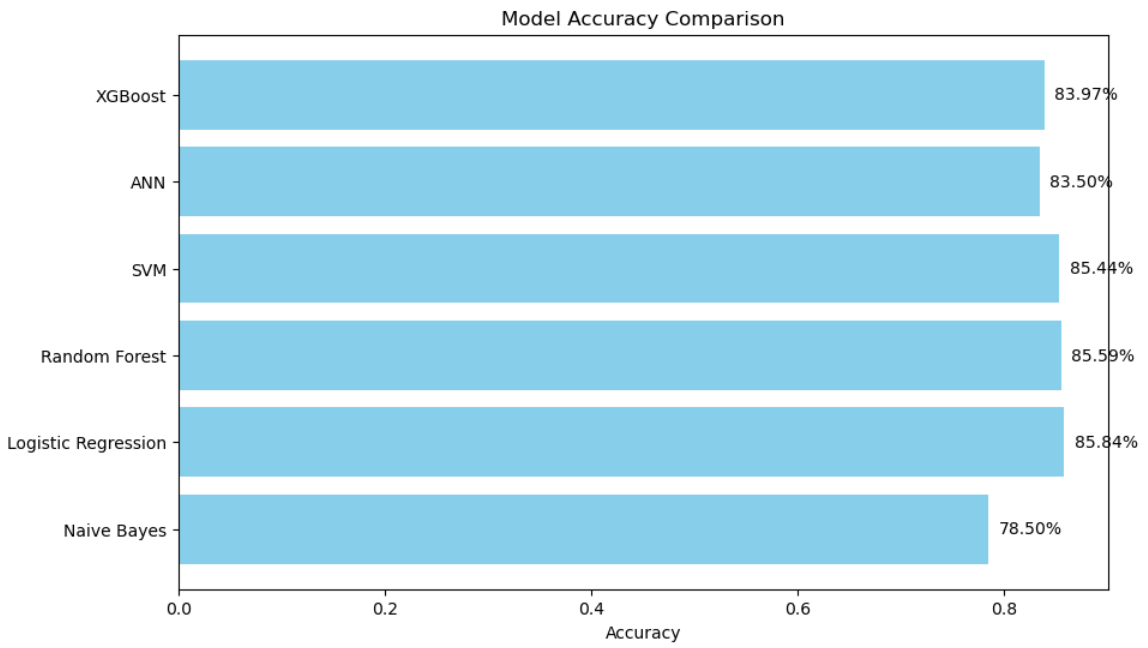
\includegraphics[width=0.8\textwidth]{model_accuracy.png}
\caption{Model Accuracy Comparison}
\label{fig:model_accuracy}
\end{figure}
As shown in Figure \ref{fig:model_accuracy}, Logistic Regression emerged as the top-performing model with an accuracy of \textbf{0.8584}. It was closely followed by Random Forest (\textbf{0.8559}) and SVM (\textbf{0.8544}). ANN achieved the lowest accuracy at \textbf{0.835}, highlighting the potential for further improvements in performance. XGBoost showed a solid accuracy of \textbf{0.8397}, rounding out the list of top models.

Logistic Regression performed exceptionally well across all emotion categories, with Random Forest and SVM also demonstrating strong results. Although ANN had the lowest accuracy, its strong recall in detecting emotions such as \textbf{Love} suggests it could be improved with further tuning. XGBoost demonstrated competitive performance but could benefit from addressing lower precision in emotions like \textbf{Surprise}. The results indicate that further optimization of hyperparameters for each model could enhance their performance, especially for less represented emotions.
